% GENERATED by scripts/make_lipics.py from paper/main.tex — edit that file, not this one.
\documentclass[a4paper,UKenglish,cleveref,autoref,thm-restate,anonymous]{lipics-v2021}
\usepackage{booktabs}
\graphicspath{{../}}
\bibliographystyle{plainurl}
\title{Pleated Ribbon Construction: Approximate Sorting Recovers the Locality of a Full Sort}
\titlerunning{Pleated Ribbon Construction}
\author{Anonymous Author}{Anonymous Affiliation}{}{}{}
\authorrunning{Anonymous}
\Copyright{Anonymous}
\ccsdesc[500]{Theory of computation~Data structures design and analysis}
\ccsdesc[300]{Information systems~Data structures}
\keywords{ribbon filter, approximate membership, filter construction, cache locality, algorithm engineering}
\supplement{Raw measurements, registered protocols and analysis scripts accompany the submission.}
\begin{document}
\maketitle
\begin{abstract}
Probabilistic membership filters let storage systems skip reads for keys that are not present. Ribbon filters use much less memory than Bloom filters at comparable false-positive rates, but their higher construction cost limits deployment. The published homogeneous ribbon algorithm sorts keys by start position, at least approximately; the reference implementation and RocksDB insert them in arrival order instead. I ask how coarse that sort can be while keeping its benefit. A counting-sort partition into cache-sized windows of start positions, with no order inside a window, keeps nearly all of a full sort's locality at about one quarter of its reorder cost. On a bare-metal server, at 100--400 million keys and over ten runs per cell, sequential construction is 1.56--1.61$\times$ faster than with the best full sort I measured and 2.47--2.57$\times$ faster than the reference build; the gain holds in eight filter configurations and on real key sets, but not when string keys are rehashed in every pass. The gain comes from reducing misses in dependent row-reduction chains; for the tested Bloom construction and filter queries, whose misses are independent, software prefetch already recovers most of what batching can.

I prove that banding followed by back-substitution produces the same filter under any insertion order, for a fixed hash seed and table size, whenever the system is consistent, which a homogeneous ribbon system always is; reordered builds matched the arrival-order build in every measured run and had no false negatives. A slot-range parallel implementation takes 15.0 ns/key at 100 million keys with 16 threads. The method also transfers to RocksDB's shipped Standard128 ribbon builder, where filter construction is $1.8\times$ faster at 100 million keys per filter, with no gain for filters that fit in cache, and measured false-positive rates match stock to six digits. In the evaluated compaction configuration, which favors filters, total compaction CPU falls by 15\%. These results apply to the evaluated filters, parameters, and machines; they do not establish a general construction or deployment crossover with Bloom.
\end{abstract}


\section{Introduction}
A membership filter is a small in-memory summary of a large key set. Ask it whether a key is present, and it answers ``definitely not'' or ``probably yes.'' The first answer is the one worth having: a database that keeps a filter in front of each data file skips reading any file whose filter says no. Bloom filters~\cite{bloom1970space} have done this for five decades, at a cost of about 44\% more memory than the theoretical minimum for a given error rate. A newer generation (xor, binary fuse, and ribbon filters) narrows that gap, to under 10\% for ribbon and under 1\% in ribbon's bumped variants~\cite{dillinger2021ribbon,dillinger2022burr}.

The new filters are static: each is built once over a fixed key set and never updated. That suits write-optimized databases, whose data files are immutable and are rewritten continuously by background compaction. But every rewrite also rebuilds the file's filter, so build speed matters as much as query speed, and building is where the new filters lose. A ribbon filter costs about four times the CPU of a Bloom filter (RocksDB measures 140 vs.\ 32 ns per key~\cite{rocksdbribbonblog}), so production systems keep Bloom as the default and reserve the space-efficient filters for data they rarely rewrite. The authors of these structures report the same cost. The parallel-BuRR authors write that ``[a] large portion of the construction time is spent on parallel sorting''~\cite{becht2024parallelburr}, and a recent proposal reports building several times slower than the best existing builders~\cite{limasset2026zor}.

The published homogeneous-ribbon algorithm already contains a remedy: it sorts the keys by start position, ``at least approximately''~\cite{dietzfelbinger2026ribbon}. The reference implementation and RocksDB do not perform that step; they insert keys in arrival order behind a prefetch pipeline. A full sort costs more than it should have to, so the question of this paper is how coarse the order can be while keeping the sort's benefit, and why. The answer is that it can be very coarse. Keys only need to be grouped into windows of start positions that fit in cache, in any order within a window, because what the order buys is locality for a chain of dependent memory accesses. Out-of-order execution and software prefetch already overlap independent stalls; they cannot overlap a chain in which each access depends on the previous one.

\subparagraph*{Contributions.}
\begin{enumerate}
\item A cache-sized partition keeps the locality of a full sort (\S\ref{sec:ribbon}). At scale, homogeneous ribbon banding runs at 0.30 instructions per cycle, stalled on dependent row-reduction chains, which prefetch cannot hide. The ribbon authors' own homogeneous-ribbon algorithm already asks for the keys to be sorted by start position ``at least approximately''~\cite{dietzfelbinger2026ribbon} (and already in its technical report~\cite{dillinger2021burrtr}) for a step-count reason, but the reference implementation and RocksDB band in arrival order, and I found no implementation or measurement of the step. I implement it as a cache-sized counting-sort partition and measure it: grouping keys into L2-sized windows of start positions, with no ordering inside a window, removes all of a full start-position sort's reduction in generic cache misses and 99.8\% of its TLB walks (SGAUSS~\cite{dietzfelbinger2019gauss}, BuRR~\cite{dillinger2022burr}), though only 85.0\% of its reduction in retired loads that miss L2, at 8.2--9.1 ns/key, where BuRR's own ips2ra sorter costs 33.9--34.3. End to end, construction is 1.56--1.61$\times$ faster than with the best full sort and 2.47--2.57$\times$ faster than the reference prefetch-pipelined build, which does not sort. The ratio to the reference is 2.28--2.66$\times$ in eight configurations of band width, result bits and space, and 2.22--2.52$\times$ on three real integer key sets and on string keys hashed once; with the string itself as the key, rehashed in every pass, there is no gain. The result is insensitive to window size: totals stay within 13\% from $2^{13}$ to $2^{20}$ slots.
\item The solved filter does not depend on insertion order (\S\ref{sec:parallel}). For any consistent system, banding and back-substitution give the same filter in every order (Proposition~\ref{prop:order}, proved in Appendix~\ref{app:proof}), even though the redundant keys that are dropped can differ; a homogeneous ribbon system is always consistent. This extends the ribbon authors' observation that the set of filled slots is order-invariant. My implementation still compares each result's FNV-1a fingerprint with the arrival-order build and checks for false negatives; the fingerprints matched in every run of every experiment reported here. A slot-range parallel variant that defers boundary keys (at most 0.23\% of them) can therefore be checked against the sequential result with a checksum: banding is 6.0$\times$ faster at 8 threads and 10.7$\times$ at 16 than sequential pleated banding. The total is 15.0 ns/key at 100M keys.
\item The technique transfers to RocksDB's shipped Standard128 ribbon builder (\S\ref{sec:rocksdb}). One counting pass makes filter construction $1.8\times$ faster at 100M keys/filter and yields $25\times$ fewer banding cache misses at the same instruction count. RocksDB's tests pass, measured false-positive rates match stock to six digits, and in a separate check, all 443 filters I compared were byte-identical to stock. In the compaction configuration I evaluated, which favors filters, total compaction CPU fell by 15\% (20 runs per arm, interval of the ratio 0.849--0.852). I also give what is, to my knowledge, the first evaluation of the construction prefetch that RocksDB ships behind a ``TODO: verify/validate'' comment (\S\ref{sec:prefetch}): it is worth 1.29--1.7$\times$ on unsorted banding across the machines I measured, and pleating recovers most of its benefit.
\item Two negative results mark where reordering does not help (\S\ref{sec:nulls}). Batched probing did not win: miss-dominated point probes are limited by the number of outstanding misses a core can sustain, and software prefetch already recovers most of what that limit allows. Cross-key SIMD batching loses to per-key probing even with every address L1-resident. Bulk Bloom construction gained little beyond what a prefetch loop gives, for the same reason: its misses are independent, so they can be overlapped. Radix-partitioned construction in the style of Schmidt et al.~\cite{schmidt2021partitioned} topped out at 1.45--1.71$\times$ over per-key insertion; a prefetch loop of the kind RocksDB ships without a published evaluation recovered most of that with no transient memory; and my read-free register-aggregated apply, the design the experiment was built around, was 1.5$\times$ slower than partitioned read-modify-write, because partitioning had already turned the target misses into L2 hits.
\end{enumerate}

The primary measurements use a bare-metal AWS c7i.metal-24xl (Intel Xeon Platinum 8488C, 48 cores, no hypervisor): single-threaded runs pinned to one core with memory, frequency and page-size settings recorded, ten repetitions per cell, reported as medians with 95\% bootstrap intervals for ratios. Bare-metal Graviton4 and AMD EPYC machines replicate the headline. Earlier experiments ran on an i9-14900HX laptop (8 performance and 16 efficiency cores) without pinning and with three repetitions; where a result comes only from that machine, I say so. Comparative numbers come from the field's reference benchmark suites, run unmodified at pinned versions: fastfilter\_cpp (whose ribbon implementations are the reference code of ribbon's creator, Peter Dillinger) and BuRR. Throughout, ``reference'' means this reference \emph{implementation}, which bands keys in arrival order behind a prefetch pipeline; it omits the approximate sort that the published homogeneous-ribbon algorithm lists~\cite{dietzfelbinger2026ribbon}. The only benchmark code I wrote for the homogeneous-kernel study is a thin driver that permutes the input order around the unmodified kernel; its parallel variant additionally uses a boundary-checked copy of the reference banding loop. Cross-machine results are in \S\ref{sec:arm}. For each experiment, the hypothesis and the rule for deciding it were written down and committed before data collection, and results that went against a prediction are reported with the others. Raw outputs and analyses are in the repository.

\section{Background}\label{sec:background}
\subparagraph*{Ribbon banding.} A ribbon filter solves a banded GF(2) system. Each key hashes to a start column $s$ and a $w$-bit coefficient row, and insertion XOR-reduces that row against the rows already stored until an empty slot absorbs it. Dietzfelbinger and Walzer showed that sorting rows by start position makes banded elimination linear (SGAUSS). For standard ribbon, the ribbon paper then made the sort optional: rows can be inserted on the fly, in arbitrary order, and ``[t]here is no need to pre-sort the keys''~\cite{dillinger2021ribbon}. RocksDB's builder and the reference implementation work this way. BuRR brought the sort back (ips2ra, by bucket) because bumping needs it. Homogeneous ribbon, the variant I target, never fails construction and stores no per-key result rows. For this variant the published algorithm is not order-free. Its construction listing in the full version of the BuRR paper~\cite{dillinger2021burrtr} has the step ``sort $S$ approximately by $s(x)$'', and the accompanying proof notes that it is enough if keys are ``sorted into buckets of $b$ consecutive starting positions each and buckets handled from left to right.'' The unified journal treatment~\cite{dietzfelbinger2026ribbon} keeps the step as ``sort $S$ by $s(x)$'', annotated ``at least approximately.'' The stated reason is a bound on the row operations spent on redundant insertions, not memory locality. That bound does not limit construction in my runs: at 100M keys, banding executes 97.4 instructions per key in arrival order, 96.2 after a full sort, and 97.8 after partitioning. Order changes where banding touches memory but not how much work it does. The same papers observe that the set of filled slots does not depend on insertion order. Coarse bucketing by start position is therefore the ribbon authors' idea. I found no implementation of it in print or in code, no cache-miss account of why it matters, and no measurement of how much of a full sort's benefit it keeps; the reference implementation I benchmark and RocksDB both band in arrival order with a prefetch pipeline. I use \emph{pleating} as a name for the cache-sized instance of that approximate sort.

\subparagraph*{What the filter stores and how a query works.} A ribbon filter is an $m \times r$ bit matrix $Z$. Hashing maps each key $k$ to three values: a start position $s(k)$, a $w$-bit coefficient row $c(k)$ whose first bit is always 1, and $r$ result bits $b(k)$. The filter represents $k$ by satisfying one linear equation over GF(2): $c(k)\cdot Z = b(k)$, with $c(k)$ occupying columns $[s(k), s(k){+}w)$. A query recomputes $s$, $c$, and $b$ and answers ``present'' if and only if $c\cdot Z = b$. A key that was never inserted passes that test by chance with probability $2^{-r}$, which is the false-positive rate; at $r = 7$, that is just under 0.8\%.

\subparagraph*{Why banding is local.} Construction solves the linear system incrementally: each insertion XOR-reduces its row against stored rows until an empty slot absorbs it. Because a key's coefficients span only $w$ consecutive columns, all of the work for that key happens in a run of slots beginning at $s(k)$, and the expected run is short~\cite{dillinger2021ribbon}. The techniques in this paper rely on that locality: grouping keys by start region confines banding's memory traffic to one region at a time, and a thread that owns a range of slots can process every key whose run stays inside it.

\subparagraph*{The homogeneous variant.} Homogeneous ribbon stores no per-key result rows during banding and never fails: a row that reduces to zero is dropped, trading a small false-positive elevation for guaranteed completion. My configuration, except in Appendix~\ref{app:eseven}, is $w = 64$, $r = 7$, and $m \approx 1.09n$ slots, which gives 7.63 bits per key at a measured false-positive rate of 0.82\%.

\subparagraph*{Binary fuse.} Binary fuse construction partially sorts keys by segment, explicitly to reduce cache misses~\cite{graf2022binaryfuse}; I measured that fix directly (plain xor: 9.45 generic hardware cache misses/key; binary fuse: 1.08). This is the closest analogue to my method outside the ribbon family: a single linear pass into coarse position buckets, motivated by cache behavior, and not a full sort. Binary fuse ships the pass as part of its published construction; the ribbon implementations I measured do not have one.

\section{Partition-instead-of-sort for ribbon}\label{sec:ribbon}
\subsection{The target, measured}
At 100 million keys on the primary machine, the reference build spends 84.8 ns per key
in banding, and the hardware counters show why: banding runs 97.8 instructions in
323 cycles per key (0.30 instructions per cycle) with 3.2
generic cache misses per key, so it spends most of its time waiting on memory. Each key starts its elimination at an
effectively random position in a 1.3\,GB table, and every reduction step needs the result of the
previous XOR before it can compute which slot it touches next. A prefetcher cannot run
ahead of such a chain. Bloom construction is the opposite case: each
key's memory accesses are independent, and the hardware overlaps them.
\subsection{Design}
I only permute the input. One counting pass buckets keys by $\lfloor s / 2^{16} \rfloor$ (windows of $2^{16}$ slots, roughly 768\,KiB of banding state, under half an L2 cache), recomputing the hash on the fly instead of materializing pairs; a second pass writes the keys out in window order. The unmodified reference kernel, including its prefetch pipeline, then consumes the permuted array. Everything downstream (banding, back-substitution, queries) is reference code, so the speedup is attributable to reordering alone. Figure~\ref{fig:order} shows the change in access pattern.

\subparagraph*{Cost in memory.} The pass is not in place. It allocates one additional array of $n$ 64-bit keys, 8 bytes per key, which is transient and is freed after banding; the window counters are negligible, and the parallel variant copies each thread's keys once more. Measured peak resident memory agrees: at 100M keys the pleated build peaks 8.0 bytes per key above the reference build, against 23.0 for the ips2ra sort in the same driver (Appendix~\ref{app:scope}, which also states what each reported time includes).
\begin{figure}
\centering
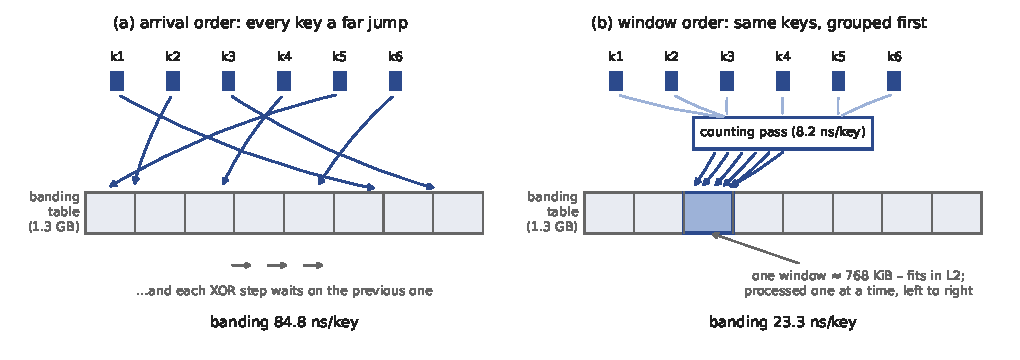
\includegraphics[width=\linewidth]{figures/banding_order.pdf}
\caption{Effect of insertion order on banding. (a) In arrival order, every key starts its
elimination at a random position in a table far larger than the L2 cache, and
the steps within each insertion form a dependent chain no prefetcher can run ahead of. (b) A
counting pass assigns keys to table windows, and a scatter pass groups them by window;
banding then works inside one
cache-resident window at a time. Binary fuse filters apply the same remedy to their counter
scatter via a segment sort (\S\ref{sec:background}). Numbers: 100M keys, primary machine, medians of 10 runs.}
\label{fig:order}
\end{figure}

\subsection{Results}
Table~\ref{tab:ribbon} gives the results at 100M keys on the primary machine, and Table~\ref{tab:scale} gives the totals at 10M, 100M, and 400M. The partition pass costs 8.2--9.1 ns/key against 33.9--34.3 for ips2ra in my driver. Banding after partitioning costs 23.3 ns/key against 19.3 after a full sort and 84.8 in arrival order. End to end, construction takes 36.1 ns/key against 89.4 for the reference and 58.3 for the best full sort (Figure~\ref{fig:strategies}): 2.47$\times$ faster than the reference (95\% interval 2.46--2.49) and 1.61$\times$ faster than the best full sort; at 400M keys, 2.57$\times$ and 1.56$\times$. At 10M keys, where much of the table fits in this machine's 105\,MB last-level cache, the gain over the reference is only 1.23$\times$.

\subparagraph*{What the miss counters show.} The generic cache-miss event falls from 3.2 to 0.26 per key, the same as after a full sort (100.0\% of the sort's reduction), and TLB walks fall by 99.8\% of the sort's reduction. Counting only retired loads that miss L2 (\texttt{mem\_load\_retired.l2\_miss}), the partition removes 85.0\% of the sort's reduction at 100M keys and 84.9\% at 400M. I had registered at least 90\% on that event, so that prediction failed. The reference build prefetches each key's start, which leaves it only 0.11 such misses per key; my reading, not tested, is that the event sees the misses the prefetch does not cover, and the partition removes fewer of those. On Graviton4 the partition removes 96.7--97.5\% of the sort's reduction in L2 read misses (\S\ref{sec:arm}). BuRR is included only as a mechanistic anchor: it uses a different, bumped structure ($r=8$, about 1\% space overhead) than my homogeneous configuration (7.63 bits/key at 0.82\% FPR, about 9.5\% overhead), so I do not compare end-to-end totals with it. On the laptop, a window sweep from $2^{13}$ to $2^{20}$ slots moved totals only between 23.8 and 26.9 ns/key, and the choice of $2^{16}$, fixed before the sweep, was conservative: $2^{14}$ is slightly faster (Appendix~\ref{app:extra}, Table~\ref{tab:sweep}). Eight other filter configurations, three real integer key sets and string keys are in Appendix~\ref{app:eseven}.

\begin{table}
\caption{Homogeneous ribbon construction on the primary machine (Xeon Platinum 8488C, bare
metal), 100M keys, ns/key: median (minimum--maximum) of 10 runs. Reorder includes allocating the
permuted array; banding and back-substitution include hashing.}
\label{tab:ribbon}
\small\setlength{\tabcolsep}{4pt}
\begin{tabular}{lrrr}
\toprule
strategy & reorder & banding & total \\
\midrule
unsorted, no prefetch & --- & 116.7 (114.8--117.7) & 121.4 (119.5--122.4) \\
unsorted + prefetch (ref.) & --- & 84.8 (84.3--86.6) & 89.4 (89.0--91.2) \\
full sort (std::sort) & 96.9 (96.7--97.5) & 19.4 (19.3--19.4) & 120.9 (120.7--121.6) \\
full sort (LSD radix) & 38.0 (37.8--38.1) & 19.4 (19.3--19.4) & 62.0 (61.8--62.1) \\
full sort (ips2ra) & 34.3 (34.1--35.4) & 19.3 (19.3--19.4) & 58.3 (58.0--59.4) \\
\textbf{partitioned (this work)} & 8.2 (8.2--8.3) & 23.3 (23.2--23.3) & 36.1 (36.1--36.2) \\
\midrule
parallel, 8 threads (this work) & 8.2 & 3.9 (3.9--3.9) & 16.7 (16.7--16.8) \\
parallel, 16 threads (this work) & 8.2 & 2.2 (2.2--2.8) & 15.0 (15.0--15.6) \\
\bottomrule
\end{tabular}
\end{table}

\begin{table}
\caption{Construction by key count on the primary machine, medians of 10 runs (ns/key), and how
many times faster the partitioned build is than the reference build and than the best full sort
(the fastest of the three sorts at that size).}
\label{tab:scale}
\begin{tabular}{rrrrrr}
\toprule
keys & reference & best sort & partitioned & vs.\ reference & vs.\ best sort \\
\midrule
10M & 43.3 & 55.6 & 35.2 & 1.23$\times$ & 1.58$\times$ \\
100M & 89.4 & 58.3 & 36.1 & 2.47$\times$ & 1.61$\times$ \\
400M & 95.4 & 57.9 & 37.0 & 2.57$\times$ & 1.56$\times$ \\
\bottomrule
\end{tabular}
\end{table}

\subparagraph*{The remaining gap to Bloom.} On the laptop, in the same harness and at close false-positive rates, ribbon
construction goes from 4.4$\times$ the cost of blocked Bloom to 2.2$\times$:
pleating roughly halves the gap but does not close it (Appendix~\ref{app:extra}, Table~\ref{tab:bloomgap}).
The comparisons against a production Bloom builder and at equal thread counts are in
\S\ref{sec:rocksdb} and \S\ref{sec:parallel}.

\begin{figure}
\centering
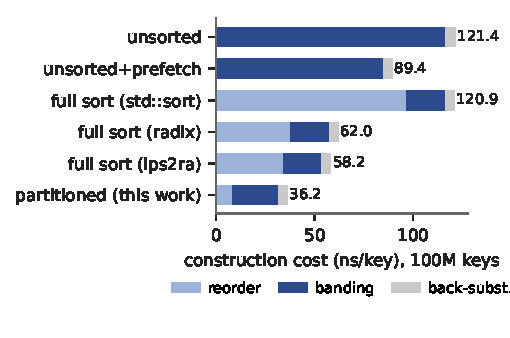
\includegraphics[width=0.85\linewidth]{figures/strategies_100m.pdf}
\caption{Construction cost by phase, 100M keys, primary machine, medians of 10 runs. The
partition pass replaces the sort at about a quarter of its reorder cost; banding after it costs
about a fifth more than after a full sort.}
\label{fig:strategies}
\end{figure}

\section{Portability across machines}\label{sec:arm}
The same protocol ran on two further bare-metal machines, a Graviton4 (Neoverse-V2) and an AMD
EPYC 9R14, as replications. Table~\ref{tab:arm} gives the totals at 100M keys, with the laptop's
earlier runs for comparison. On Graviton4 the partitioned build is 2.17$\times$
and 2.27$\times$ faster than the reference at 100M and 400M keys, and
1.29$\times$ and 1.30$\times$ faster than the best full sort,
and it removes 96.7\% and 97.5\% of the sort's reduction in L2 read
misses (\texttt{l2d\_cache\_lmiss\_rd}). On the AMD machine the figures are 2.05$\times$ and 2.35$\times$ over the reference, 1.33$\times$ and 1.23$\times$ over the best full sort, and 96.4\% and 96.6\% of the sort's reduction in data-cache misses in L2 (\texttt{l2\_cache\_req\_stat.ic\_dc\_miss\_in\_l2}). The gain over the best full sort is smaller on both replications than on the Xeon, where the sorts are slower. Earlier, unpinned runs on an Ampere Altra
(Neoverse-N1) and a Google Axion (Neoverse-V2) with three repetitions each gave 2.37$\times$ and
2.72$\times$ over the reference.

The output checks passed on every machine: zero false negatives, and in every repetition every
strategy produced the same 64-bit FNV-1a solution fingerprint as the arrival-order build. These
are hash comparisons, not bytewise comparisons, and the order-related part is what
Proposition~\ref{prop:order} predicts.

\begin{table}
\caption{Construction across machines, 100M keys, ns/key. Bare-metal rows: medians of 10 runs,
pinned. Laptop row: medians of 3 earlier, unpinned runs.}
\label{tab:arm}
\small\setlength{\tabcolsep}{4pt}
\begin{tabular}{lrrrrr}
\toprule
machine & reference & best sort & partitioned & vs.\ reference & vs.\ best sort \\
\midrule
Xeon 8488C (Intel) & 89.4 & 58.3 & 36.1 & 2.47$\times$ & 1.61$\times$ \\
EPYC 9R14 (AMD) & 82.0 & 53.0 & 40.0 & 2.05$\times$ & 1.33$\times$ \\
Graviton4 (Arm) & 76.9 & 45.7 & 35.5 & 2.17$\times$ & 1.29$\times$ \\
i9-14900HX laptop (3 reps, not pinned) & 48.9 & 40.6 & 24.1 & 2.03$\times$ & 1.69$\times$ \\
\bottomrule
\end{tabular}
\end{table}

\section{Order-independence and parallel construction}\label{sec:parallel}
\begin{proposition}[Order-independence]\label{prop:order}
Let $E=\{(r_k,b_k)\}$ be a consistent system of equations over $\mathrm{GF}(2)$ in $m$ unknowns,
for one fixed hash seed and table size, each $r_k$ carrying a leading 1 at its start position. Then banding (reduce each row against the stored
rows, store it at the slot of its leading position, and drop it if it reduces to zero) followed
by back-substitution in which every free slot $j$ is assigned a value $g(j)$ that depends only
on $j$ (not on the table's contents or on the insertion history) yields the same solution $Z$
under every insertion order of $E$.
\end{proposition}
The rows need not be linearly independent. A homogeneous ribbon system has $b_k=0$ for every key
and is therefore always consistent, so a homogeneous ribbon filter does not depend on insertion
order at all. In the kernels I use, a standard ribbon build for a given seed fails only when a
row reduces to zero with a nonzero right-hand side, so it succeeds exactly when its system is
consistent, and that too is a property of $E$, not of the order: if $E$ is inconsistent, every
order meets such a row. The proposition does not cover schemes that bump or give up on keys
depending on their position in the order, as BuRR does.

The first step of the proof is known: the ribbon papers state that the set of filled slots is
invariant under insertion order~\cite{dillinger2021ribbon,dietzfelbinger2026ribbon}. I extend
that observation to the solved filter; the proof, which is elementary linear algebra, is in
Appendix~\ref{app:proof}. The measurements agree: across every homogeneous sequential and parallel
run (sizes up to 400 million keys, six reordering strategies, up to 16 threads) the finished filter's
64-bit FNV-1a fingerprint matched the arrival-order build, and all 443 RocksDB standard ribbon
filters I compared were byte-identical to stock (\S\ref{sec:rocksdb}). I keep the per-run
fingerprint comparison in the implementation as a guard against bugs, not because the result
depends on it. My parallel version assigns disjoint window ranges
(split at the same key count) to threads; keys starting within $2^{14}$ slots of a range boundary switch
to a sequential tail (at most 0.23\% of keys), following the boundary handling of parallel BuRR. BuRR makes shards independent by bumping every key whose equation spans a shard boundary to the next layer~\cite{dietzfelbinger2026ribbon,becht2024parallelburr}; a ribbon without bumping has no next layer, so I defer those keys within the same system instead. Safety does not rest on that margin: a thread never writes at or beyond the upper boundary of its range, and a reduction that would reach it is handed to the sequential tail instead (Appendix~\ref{app:scope}). On the primary machine,
banding at 16 threads is 12.9$\times$ faster than the parallel path's own single-thread run (Figure~\ref{fig:scaling})
and 10.7$\times$ faster than sequential pleated banding (6.0$\times$ at 8 threads); the parallel path carries
about 20\% overhead for deferring and copying keys. The counting pass
(8.2 ns/key) and
back-substitution (4.6 ns/key) remain sequential and together
account for most of the 15.0 ns/key total. Both can be parallelized, the counting sort directly and back-substitution as in parallel BuRR; I leave both to future work.

\subparagraph*{Against Bloom at equal thread counts.} Bloom insertion is order-free and parallelizes with
little effort, so a 16-thread ribbon build should be compared with a 16-thread Bloom build. On a
16-core machine, pleated ribbon costs 4.0$\times$ the best
Bloom build at one thread and 10.1$\times$ at 16. The gap widens because only banding is
parallel in my build (Appendix~\ref{app:efour}, Table~\ref{tab:efour}).
\begin{figure}
\centering
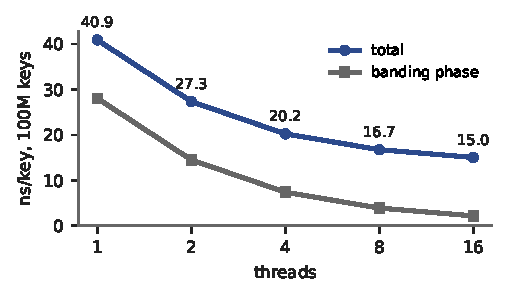
\includegraphics[width=0.85\linewidth]{figures/parallel_scaling.pdf}
\caption{Slot-range parallel construction, 100M keys, primary machine, medians of 10 runs; every
run has a matching 64-bit solution fingerprint against the sequential build.}
\label{fig:scaling}
\end{figure}


\section{Construction prefetch, evaluated}\label{sec:prefetch}
RocksDB ships a software-pipelined construction prefetch behind a comment reading ``TODO: verify/validate'', and the reference harness enables the same pipeline above 1500 slots. My no-prefetch control isolates its effect on unsorted banding at 100M keys: 1.38$\times$ on the primary machine (116.7 $\to$ 84.8 ns/key), 1.29$\times$ on Graviton4, and 1.5--1.7$\times$ on the laptop. The prefetch removes the miss that locates a key's start but cannot shorten the dependent reduction chain, which is why partitioning dominates here while a similar prefetch strategy wins for Bloom construction (\S\ref{sec:nulls}).

\section{Pleating a production engine: RocksDB}\label{sec:rocksdb}
The ribbon measurements so far use a reference-kernel harness on homogeneous $w=64$ ribbon. The filter that
RocksDB ships is different: \texttt{Standard128RibbonBitsBuilder}, a
\emph{standard} ribbon at $w=128$~\cite{rocksdbribbonblog}. I therefore tested whether
pleating transfers to it in RocksDB's own build path. The patch is one
counting pass over the collected key hashes, inserted immediately before RocksDB's banding call
(\texttt{ResetAndFindSeedToSolve}); everything downstream is unmodified engine code. As written, the patch is not in place: it holds a second copy of the collected 64-bit hashes and a 32-bit window index per key, 12 bytes (96 bits) per key of transient memory, where RocksDB reports about 230 bits per key of temporary memory for ribbon construction~\cite{rocksdbribbonblog}. In \texttt{filter\_bench} at 100M keys per filter the process peaks at 4.6~GiB with the pass and 3.6~GiB without (Appendix~\ref{app:scope}). An integration meant for upstream would need to reduce that and to bypass the pass for small filters. Proposition~\ref{prop:order}
applies to this builder one seed at a time: whether a seed succeeds does not depend on order, so
the same seed is selected, and the solution for that seed is the same (\S\ref{sec:parallel}). This
depends on where the pass is placed. RocksDB derives the starting seed and the filter length from the
first collected hash, and my reorder runs after both are fixed; a reorder placed earlier could
change them. I also tested the output directly. RocksDB's own filter tests pass unchanged, and the
measured false-positive rate matches stock to six digits at every reported size. That gate
alone does not establish bit identity, so I checked identity directly in a separate
experiment: the same binary dumps every finished filter, and I compared stock and pleated
output byte by byte at 100K, 1M, 10M, and 100M keys per filter, with a second stock run as a
determinism control. All 443 filters were byte-identical, and the control matched. The comparison covers the stored metadata, including the hash seed, so the same seed was selected in every case, and byte-identical filters answer every query identically. This holds for
the filters built in that experiment; it is not a proof for all inputs. Every measurement first confirms that the binary contains the patch (object recompiled, binary newer
than source, marker string present), because an early build failure had left a stale stock binary
in place.

\subparagraph*{Construction microbenchmark} (\texttt{filter\_bench}, the engine's own tool; 10 bits/key).
Table~\ref{tab:rocksdb} reports total filter-construction cost, while Figure~\ref{fig:rocksdb}
plots the banding phase alone. At 100M keys per filter, pleating builds RocksDB's ribbon
$1.8\times$ faster overall. The pleated build cost is nearly flat with filter size (54.4--55.5 ns/key
from 1M to 100M keys), while the stock build cost rises from 55.9 to
97.4 ns/key as the banding table outgrows the cache. Below the cache crossover (a filter of $10^5$ keys
fits in cache), pleating is a few percent \emph{slower} because the counting pass has a cost and
there is no locality to recover, as the mechanism predicts.

\subparagraph*{Mechanism.} The cause is the same dependent-miss chain, which I confirm with hardware
counters scoped to RocksDB's banding call. At 100M keys, pleating reduces banding cache misses from
11.5 to 0.47 per key (a $25\times$ reduction) while the instruction count is unchanged (243 per
key in both builds). The work is the same; the working set now fits
in cache. The time speedup is smaller than for $w=64$ because the standard $w=128$ kernel does more computation per key, and pleating largely subsumes RocksDB's construction prefetch (Appendix~\ref{app:extra}).

\subparagraph*{End-to-end during compaction.} In \texttt{db\_bench} on the primary machine (30M keys
of 16 bytes with 8-byte values, so that filters are a large share of compaction work; 256\,MiB
SST target), total compaction CPU falls from 9.42 to 8.01 seconds,
by 15\% (20 runs per arm, interval of the ratio
0.849--0.852). The reduction is smaller with 64\,MiB SSTs and larger with 1\,GiB SSTs
(Appendix~\ref{app:eseven}, Table~\ref{tab:esevencomp}): it grows with the size of each SST's
filter. Configurations with larger values make filters a smaller share and would show less.

\begin{table}
\caption{Pleating RocksDB's shipped Standard128 ribbon (\texttt{filter\_bench}, 10 bits/key,
 i9-14900HX laptop; means of 3). The measured false-positive rate matches stock to six digits at every size.
Banding generic hardware cache misses/key from counters scoped to the banding call.}
\label{tab:rocksdb}
\begin{tabular}{lrrr}
\toprule
keys/filter & stock ns/key & pleated ns/key & speedup \\
\midrule
$10^5$ (cache-resident) & 57.6 & 59.4 & 0.97$\times$ \\
$10^6$                  & 55.9 & 54.4 & 1.03$\times$ \\
$10^7$                  & 88.7 & 54.7 & 1.62$\times$ \\
$10^8$                  & \textbf{97.4} & \textbf{54.8} & \textbf{1.78$\times$} \\
\midrule
banding misses/key @$10^8$ & 11.5 & 0.47 & --- \\
\bottomrule
\end{tabular}
\end{table}

\subparagraph*{Against RocksDB's own Bloom.} At a matched false-positive rate in the same harness, the
pleated builder costs 2.4$\times$ RocksDB's production Bloom builder at 100M keys per filter, down
from 4.5$\times$ for stock; below the cache crossover, pleating does not help. That
experiment, on a second x86 machine, is in Appendix~\ref{app:ethree} (Table~\ref{tab:ethree}).
\begin{figure}
\centering
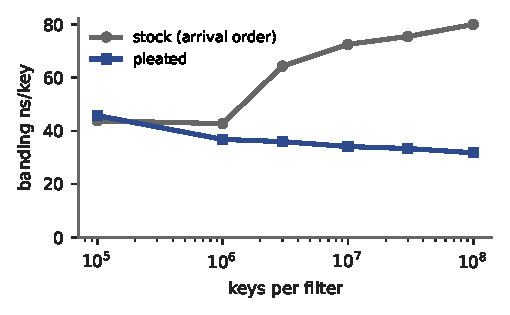
\includegraphics[width=0.85\linewidth]{figures/rocksdb_scale.pdf}
\caption{RocksDB Standard128 ribbon banding-phase cost vs.\ filter size. Pleated banding cost does not
rise (cache-resident per window); stock banding degrades as the table outgrows cache. Measured
false-positive rates match stock to six digits at every point.}
\label{fig:rocksdb}
\end{figure}

\section{Where reordering does not help}\label{sec:nulls}
This section reports two optimizations that failed. Each was tested under favorable conditions, with its protocol fixed before any run: the batched probe was timed with every address already in cache, and the read-free builder was the design its experiment was built around. Both lost. An optimization that cannot win under conditions chosen to favor it points to a limit of the hardware and not of the setup.

\subsection{Point probes are MLP-bound}
I compared probe strategies over identical split-block Bloom filters (Parquet geometry), 32\,KiB up to 512\,MiB (the instrument was amended once after a first run; the data reported are from the amended run). My vertical, lane-structured batch probe auto-vectorizes from plain Rust to packed SIMD, yet it loses. It loses to per-key probing at every size: to plain scalar probing up to 4\,MiB, and to scalar probing with software prefetch at RAM sizes. Even with every address forced L1-hot it reaches 555 Mops/s against 665 for scalar probing at 32\,KiB, because a split-block check is already SIMD within a single key, and an AVX2 gather cannot beat eight independent scalar loads that the out-of-order window overlaps at no cost. At RAM scale, the identical instruction stream runs 5--6$\times$ faster when L1-hot, so probing is bound by memory-level parallelism. Software prefetch recovers part of that and then plateaus (148 Mops/s at 64\,MiB against 89 without it), which is what a limit on the misses one core can keep outstanding would produce. No compute bottleneck remains for a layout change to remove.

\subsection{Blocked-Bloom construction is prefetch-hidable}
I measured five bulk builders at 1M to 429M keys, each required to produce bit-identical output (OR is commutative, so any deviation is a bug). Per-key insertion does degrade at scale (one random read-modify-write miss per key, 11.5 ns/key at 100M, IPC 0.48), so there is a cost to recover. Most attempts to recover it failed. Radix-partitioned construction after Schmidt et al.~\cite{schmidt2021partitioned} reached only 1.45--1.71$\times$. A software-pipelined prefetch insert, the shape RocksDB ships, reached 6.1--8.9 ns/key with no transient memory and beat partitioning up to 100M keys. The variant this experiment was designed around is a read-free apply that partitions pre-merged (block, mask) pairs, OR-aggregates each block in registers, and issues one store per block without reading filter memory. It was 1.5$\times$ slower than partitioned read-modify-write, and non-temporal stores made no difference. The explanation is that partitioning had already turned the expensive misses into L2 hits, so the extra grouping pass spent time to save cheap loads. Bloom construction misses are independent, and the memory system already hides independent misses.

\section{Related work}\label{sec:related}
Sorted banded elimination: Dietzfelbinger and Walzer~\cite{dietzfelbinger2019gauss}, BuRR~\cite{dillinger2022burr}, and parallel BuRR~\cite{becht2024parallelburr}; the unified journal treatment of standard, homogeneous, and bumped ribbon is Dietzfelbinger et al.~\cite{dietzfelbinger2026ribbon}. Approximate sorting of homogeneous-ribbon input into buckets of consecutive start positions is specified there and in the BuRR technical report~\cite{dillinger2021burrtr}, with a row-operation bound as its rationale (\S\ref{sec:background}). Arbitrary-order banding and production engineering: ribbon~\cite{dillinger2021ribbon}, RocksDB~\cite{rocksdbribbonblog}. Cache-conscious filter design: buffered Bloom filters~\cite{canim2010buffered}, radix-partitioned filters~\cite{schmidt2021partitioned}, binary-fuse segment sort~\cite{graf2022binaryfuse}, and xor-filter buffered scatter~\cite{graf2020xor}; sharding the structure itself for construction locality in hypergraph-based static functions~\cite{genuzio2016fast,vigna2025sharding} and sort-based cache-oblivious peeling~\cite{belazzougui2013peeling}; the generic two-phase partition-then-accumulate pattern appears as propagation blocking~\cite{beamer2017propagation} with write-combining from Wassenberg and Sanders~\cite{wassenberg2011radix}. SIMD probe-side layout: Polychroniou and Ross~\cite{polychroniou2014vectorized}, Lang et al.~\cite{lang2019performance}, split-block Bloom~\cite{apache2021sbbf}. The ordering idea is therefore not mine. What was open is how coarse the order may be, what it costs, and why it works. BuRR sorts fully (ips2ra) to enable threshold-based bumping and tighter space, and bumping needs that order, so I make no claim that a coarse partition transfers to BuRR. For homogeneous ribbon, the authors specify an approximate sort, but the implementations I found do not perform one. I build it as a counting-pass partition sized to the cache, show that it keeps nearly all of the sort's locality at about a quarter of the reorder cost, explain the gain by dependent-miss chains, and apply the same pass to RocksDB's standard ribbon builder, whose design forgoes sorting. Unlike sharding, the partition only permutes the input and leaves the stored structure unchanged, which makes the transformation and its parallelization checkable against the arrival-order build.

\section{Limitations and threats to validity}\label{sec:limits}
Miss counts differ by event and by machine, so I compare reductions within a machine and do not pool absolute counts; on the primary machine the event that counts retired loads missing L2 shows a smaller recovery (85.0\%) than the generic event and TLB walks, against my registered prediction. The headline comes from one primary machine with two bare-metal replications; the window sweep, the Bloom comparisons and the RocksDB microbenchmark come from earlier, unpinned runs with three repetitions. With string keys rehashed in every pass, partitioning does not help (0.79--1.04$\times$); it pays when keys are hashed to fixed-width values once, as RocksDB does. I accelerate the \emph{homogeneous} ribbon (about 9.5\% space overhead at $r=7$), whereas BuRR has under 1\% overhead; BuRR is a mechanistic anchor, not a like-for-like baseline. The sort baselines use BuRR's sequential ips2ra but not its parallel form. The partition pass needs transient memory (8 bytes per key in the standalone driver, 12 in the RocksDB patch); peak memory and concurrent builds were measured on one machine only, with separate processes standing in for an engine's concurrent compactions. Only banding is parallelized, and the scaling ratios are against the parallel path's own single-thread run. The order-independence proposition covers systems that are solved exactly for one fixed seed and table size; it says nothing about schemes that bump keys by their position in the order. The fingerprint comparisons test the implementations against it, not the proposition itself. The RocksDB construction gain is measured on the production $w=128$ kernel; byte identity with stock is shown for the 443 filters I compared, not for all inputs. The whole-compaction result comes from a configuration that favors filters and depends on SST sizing.

\section{Conclusion}
On the measured machines, a counting-sort partition keeps nearly all of a full sort's locality for homogeneous ribbon construction at about a quarter of the reorder cost, and makes construction 2.47--2.57$\times$ faster than the reference build at 100--400M keys on the primary machine. Reordering does not change the output: for a fixed hash seed and table size, the solved filter is the same in every insertion order for any consistent system, which covers every homogeneous build and every successful standard build, and the measured fingerprints agree. The method also speeds up RocksDB's shipped $w=128$ ribbon builder by $1.8\times$ at 100M keys per filter. RocksDB's tests pass, measured false-positive rates match stock to six digits, and all 443 stock and pleated filters compared in a separate experiment were byte-identical. In a compaction configuration that favors filters, total compaction CPU falls by 15\%. Against RocksDB's own Bloom builder at a matched false-positive rate, pleated ribbon still costs 2.4$\times$ as much to build at 100M keys per filter (4.5$\times$ for stock) on one thread. In a separate equal-thread comparison of homogeneous ribbon with my blocked-Bloom prototype, not matched on space or false-positive rate, the gap grows from 4.0$\times$ at one thread to 10.1$\times$ at 16, because only banding is parallel in my build. These results hold for the evaluated filters and machines; they narrow ribbon's single-thread build-cost gap to Bloom but do not close it.

\paragraph*{Artifacts.}
All protocols, amendments, raw measurements, and integrity tooling are in the accompanying
repository. \texttt{reproduce.sh} re-derives every analysis from committed raw
measurements, checks the Rust tests and artifact integrity, and regenerates figures. It does not
rerun the measurements themselves; the registered protocols and runners for those are in the
repository. A production implementation exists; its link is withheld for double-blind review.

\bibliography{refs}

\appendix
\section{Proof of Proposition~\ref{prop:order}}\label{app:proof}
\subparagraph*{Setting.} The unknown is $Z\in\mathrm{GF}(2)^{m\times r}$. Each equation is a pair
$(r_k,b_k)$ of a nonzero row $r_k\in\mathrm{GF}(2)^m$ and a result $b_k\in\mathrm{GF}(2)^r$, and
asks for $r_kZ=b_k$. Write $\mathrm{lead}(v)$ for the first nonzero position of a nonzero row $v$.
Banding keeps a table in which slot $i$ is empty or stores a pair $(\rho_i,\beta_i)$ with
$\mathrm{lead}(\rho_i)=i$. To insert $(\rho,\beta)$: while $\rho\neq 0$ and slot
$\mathrm{lead}(\rho)$ is occupied, add that slot's pair to $(\rho,\beta)$, which moves
$\mathrm{lead}(\rho)$ strictly to the right; then store the pair at slot $\mathrm{lead}(\rho)$ if
$\rho\neq 0$, and drop it otherwise. Stored pairs are never modified. Back-substitution visits the
slots from $m$ down to $1$, setting $Z_j=g(j)$ for an empty slot $j$ and
$Z_i=\beta_i+\sum_{j>i}\rho_{i,j}Z_j$ for an occupied slot $i$, where $Z_j$ is row $j$ of $Z$.
Let $V=\mathrm{span}\{r_k\}$ and $P(V)=\{\mathrm{lead}(v) : v\in V,\ v\neq 0\}$. Vectors with
distinct leading positions are linearly independent, and every subspace has a basis in echelon
form, so $|P(V)|=\dim V$.

\emph{Proof.} Fix any insertion order and consider the table after the last insertion.

\emph{(i) The occupied slots are exactly $P(V)$.} Every stored pair is a sum of equations of $E$,
so every stored row lies in $V$. The stored rows have distinct leading positions, so they are
linearly independent. Each $r_k$ equals the remainder it was reduced to, which is zero or a stored
row, plus the stored rows that were added to it; hence the stored rows span $V$ and form a basis
of it. The occupied slots are therefore $\dim V$ distinct elements of $P(V)$, which has $\dim V$
elements. This step is the invariance of the set of filled slots that the ribbon papers
state~\cite{dillinger2021ribbon,dietzfelbinger2026ribbon}.

\emph{(ii) The stored system has the same solutions as $E$.} A solution of $E$ satisfies every sum
of equations of $E$, so it satisfies the stored system. Conversely, an equation $(r_k,b_k)$ that
was stored after reduction is the sum of its stored remainder and other stored pairs, so the
stored system implies it. An equation that was dropped satisfies $r_k=\sum_{i\in I}\rho_i$ and
$b_k=\beta'+\sum_{i\in I}\beta_i$ for a set $I$ of occupied slots, where $\beta'$ is the result it
was left with. Since $E$ is consistent, it has a solution $Z^0$, which also satisfies the stored
system, so $b_k=r_kZ^0=\sum_{i\in I}\rho_iZ^0=\sum_{i\in I}\beta_i$ and $\beta'=0$. The dropped
equation is thus a sum of stored equations, and the stored system implies it as well.

\emph{(iii) The output is determined by $E$.} By the recursion that defines it, the output $Z$ of
back-substitution satisfies every stored equation and has $Z_j=g(j)$ for every empty slot $j$; by
(i) and (ii) it is a solution of $E$ with $Z_j=g(j)$ for all $j\notin P(V)$. There is only one
such solution: two of them agree on all rows outside $P(V)$, both satisfy the stored system, and
the stored equation at slot $i$ determines row $i$ from rows $j>i$, so they agree on every row by
induction from $m$ downwards. The solution set of $E$, the set $P(V)$, and $g$ do not depend on
the insertion order, so neither does $Z$. \hfill$\square$

\subparagraph*{Remarks.} Which equations are dropped does depend on the order, as the ribbon authors
note~\cite{dietzfelbinger2026ribbon}; the solution does not. If $E$ is inconsistent, every order
meets a row that reduces to zero with a nonzero result: otherwise every dropped equation would be
a sum of stored equations, as in (ii), and the stored system, being in echelon form, has a
solution, which would then solve $E$. So whether a standard ribbon build succeeds for a given seed
is also independent of the order. The reference implementation meets the condition on $g$: it
fills free solution rows with a fixed multiplicative hash of the slot index, as the ribbon authors
describe~\cite{dietzfelbinger2026ribbon}; zero is the special case $g\equiv 0$.

\subparagraph*{Tests of the implementations.} The proposition is about the abstract procedure; whether a
given kernel implements that procedure is a separate question, which I tested. On the unmodified
reference kernel, homogeneous filters sized so that up to half of the keys are dropped as
redundant came out identical under 25 shuffled orders, and standard builds either succeeded
identically in every order or failed in every order. As a check on the statement itself, an
exhaustive enumeration of all small systems (up to seven slots and five or six equations, every
insertion order) found no violation.

\section{Bloom and ribbon in RocksDB at matched false-positive rate}\label{app:ethree}
Table~\ref{tab:rocksdb} compares
ribbon with ribbon. To compare both with Bloom, I ran a further experiment:
\texttt{filter\_bench} building RocksDB's production Bloom filter
(\texttt{format\_version} 5, which ships its own construction prefetch) and Standard128 ribbon,
stock and pleated, from the same key stream at the same bits-per-key setting, three repetitions,
arms interleaved. RocksDB sizes its ribbon to the Bloom filter's false-positive rate, so the arms
are matched by construction: measured rates were 0.96--0.97\% for Bloom and 0.95--0.96\% for
ribbon, with ribbon storing 27--30\% fewer bits per key. This run used a different machine from
Table~\ref{tab:rocksdb} (AMD EPYC-Milan, 8 dedicated vCPUs under KVM), so its absolute numbers are
not comparable with that table; all three arms ran there in one session.
Table~\ref{tab:ethree} gives the result. At 100M keys per filter, the pleated builder costs
2.4$\times$ the Bloom builder, down from 4.5$\times$ for stock; at 10M it is 4.1$\times$, down from
7.3$\times$. Below the cache crossover pleating does not help (5.2$\times$ against 5.0$\times$ at
100K). I had written down two predictions in advance. The first, that pleated ribbon would remain
more than 1.5$\times$ Bloom at 10M keys and above, holds. The second, that it would come within
1.25$\times$ of Bloom at 100M, fails, as I expected. At one thread and matched accuracy,
pleating therefore narrows ribbon's build-cost gap to Bloom and leaves a factor of 2.4 at the largest size.
Part of the narrowing at 100M is Bloom's own cost rising with filter size on this machine (15.9 to
37.1 ns/key). The stock-to-pleated speedup replicates on this second x86 machine: 1.77$\times$ at
10M and 1.86$\times$ at 100M.

\begin{table}
\caption{RocksDB \texttt{filter\_bench} build cost (ns/key, means of 3) for the production Bloom
filter and Standard128 ribbon, stock and pleated, at 10 bits/key setting (AMD EPYC-Milan, 8 dedicated vCPUs, KVM). Last column: measured
false-positive rate \%, Bloom / ribbon.}
\label{tab:ethree}
\begin{tabular}{rrrrrrr}
\toprule
keys/filter & Bloom & stock & pleated & stock/Bloom & pleated/Bloom & FP\% \\
\midrule
100,000 & 15.9 & 78.9 & 82.2 & 5.0$\times$ & 5.2$\times$ & 0.97 / 0.95 \\
1,000,000 & 20.2 & 94.2 & 83.4 & 4.7$\times$ & 4.1$\times$ & 0.97 / 0.95 \\
10,000,000 & 22.6 & 164.6 & 92.9 & 7.3$\times$ & 4.1$\times$ & 0.96 / 0.96 \\
100,000,000 & 37.1 & 167.8 & 90.3 & 4.5$\times$ & 2.4$\times$ & 0.97 / 0.95 \\
\bottomrule
\end{tabular}
\end{table}

\section{Bloom and ribbon at equal thread counts}\label{app:efour}
A 16-thread ribbon build should be compared with
a 16-thread Bloom build, and Bloom insertion is order-free, so it parallelizes with little effort.
I ran that comparison on one machine in one
session: an AWS c7a.4xlarge (AMD EPYC 9R14, 16 physical cores), 100M keys. The Bloom side is my
blocked-Bloom prototype with three parallel builders (block-range partitioning, atomic ORs on a
shared filter, and per-range scanning), each checked for a matching output fingerprint against per-key insertion; at
each thread count I take the fastest, so the baseline is the strongest I could build. The ribbon
side is the unmodified driver of Table~\ref{tab:ribbon}. Table~\ref{tab:efour} gives the result.
At one thread, ribbon costs 4.0$\times$ the best Bloom build; at 16 threads, it costs
10.1$\times$ (22.2 against 2.20~ns/key). The gap widens with
threads because my build parallelizes only banding: on this machine the sequential counting pass
and back-substitution alone cost about 20~ns/key, and the ribbon total improves 1.8$\times$ from
1 to 16 threads, where Bloom improves 4.6$\times$. Both predictions I had written down in advance
held: ribbon stays above 1.5$\times$ Bloom at every thread count, and it does not come within
1.25$\times$ at 16 threads. This comparison is not matched on space or false-positive rate (Bloom
at 10 bits/key and 1.27\% measured false positives, ribbon at 7.63 bits/key and 0.83\%), and the
prototype's sequential build is 22\% slower than the reference suite's blocked Bloom on this
machine, inside the 25\% tolerance I had set for using its numbers. Parallel banding alone is therefore not enough: closing the equal-thread gap would also require parallelizing the counting pass and
back-substitution.

\begin{table}
\caption{Equal-thread construction cost at 100M keys (AWS c7a.4xlarge, AMD EPYC 9R14, 16 physical cores). Bloom: the fastest of three parallel
blocked-Bloom builders at that thread count (10 bits/key; Criterion mean). Ribbon: pleated
homogeneous ribbon total (mean $\pm$ sample stdev of 3; sequential build at one thread).}
\label{tab:efour}
\begin{tabular}{rlrrr}
\toprule
threads & best Bloom builder & Bloom ns/key & ribbon ns/key & ribbon/Bloom \\
\midrule
1 & par\_scan\_t1 & 10.01 & $40.30\pm0.05$ & 4.0$\times$ \\
2 & par\_scan\_t2 & 8.14 & $33.89\pm0.22$ & 4.2$\times$ \\
4 & par\_range\_t4 & 5.47 & $27.09\pm0.15$ & 5.0$\times$ \\
8 & par\_range\_t8 & 3.30 & $23.83\pm0.03$ & 7.2$\times$ \\
16 & par\_atomic\_t16 & 2.20 & $22.15\pm0.07$ & 10.1$\times$ \\
\bottomrule
\end{tabular}
\end{table}

\section{Configurations, key sets, and compaction on the primary machine}\label{app:eseven}
These measurements come from the same protocol as Table~\ref{tab:ribbon}: bare-metal Xeon
Platinum 8488C, one pinned core, hypotheses and thresholds committed before data. The driver is
a generalization of the one behind Table~\ref{tab:ribbon} (band width and result bits as
compile-time parameters, slot overhead as an argument, keys from files); before any of its
numbers were used it had to reproduce that driver's solution fingerprints and false-positive
rates in every run and its median totals within 5\%, which it did within 1.1\%.

\subparagraph*{Configurations} (Table~\ref{tab:esevenconfig}). The reference build costs
2.28--2.66$\times$ the partitioned build in every configuration of band
width, result bits, and slots per key. Slots per key follow the reference suite's sizing rule
for homogeneous ribbon except in the two rows at 1.05 and 1.15.

\begin{table}
\caption{Configurations, 100M synthetic keys, primary machine; ns/key, medians of 5 runs.
FPR and bits/key are measured.}
\label{tab:esevenconfig}
\small\setlength{\tabcolsep}{3.5pt}
\begin{tabular}{rrrrrrrrr}
\toprule
$w$ & $r$ & slots/key & FPR\% & bits/key & reference & ips2ra & partitioned & ref./part. \\
\midrule
64 & 7 & 1.050 & 2.1588 & 7.35 & 101.6 & 64.6 & 42.2 & 2.41$\times$ \\
64 & 7 & 1.090 & 0.8216 & 7.63 & 90.0 & 57.6 & 35.7 & 2.52$\times$ \\
64 & 7 & 1.150 & 0.7829 & 8.05 & 80.6 & 54.2 & 32.7 & 2.46$\times$ \\
64 & 8 & 1.094 & 0.4140 & 8.75 & 89.9 & 57.9 & 35.9 & 2.50$\times$ \\
64 & 16 & 1.125 & 0.0031 & 18.00 & 89.5 & 60.7 & 39.2 & 2.28$\times$ \\
128 & 7 & 1.045 & 0.8086 & 7.31 & 161.5 & 77.9 & 60.8 & 2.66$\times$ \\
128 & 8 & 1.047 & 0.4027 & 8.38 & 161.2 & 78.2 & 61.1 & 2.64$\times$ \\
128 & 16 & 1.063 & 0.0018 & 17.00 & 159.9 & 80.9 & 64.2 & 2.49$\times$ \\
\bottomrule
\end{tabular}
\end{table}

\subparagraph*{Key sets} (Table~\ref{tab:esevenkeys}). Three integer sets from the SOSD
benchmark (Facebook user ids, OpenStreetMap cell ids, Wikipedia edit timestamps; 100M distinct
keys sampled from each, 90M for the Wikipedia set, which has no more distinct keys), the first
100M host names of a Common Crawl host graph, and random strings of 16 and 64 bytes. Strings are
measured two ways. Hashed once with XXH3 to 64 bits, as RocksDB does, the hashing is timed and
counted in the total, and the partition then works on fixed-width values: the reference build
costs 2.22--2.52$\times$ the partitioned build. With the string itself as the
filter's key, the hash is recomputed in each partition pass and again in banding, and banding
reads strings in an order that follows the table, not the storage: then the partition does not
pay (0.79$\times$ to 1.04$\times$).

\begin{table}
\caption{Key sets, primary machine; ns/key including hashing, medians of 5 runs. Hash: the
once-only XXH3 phase.}
\label{tab:esevenkeys}
\small\setlength{\tabcolsep}{3.5pt}
\begin{tabular}{lrrrrrr}
\toprule
keys & count & bytes & hash & reference & partitioned & ref./part. \\
\midrule
SOSD Facebook ids & 100M & 8.0 & 0.0 & 89.8 & 35.6 & 2.52$\times$ \\
SOSD OSM cell ids & 100M & 8.0 & 0.0 & 89.7 & 35.6 & 2.52$\times$ \\
SOSD Wikipedia timestamps & 90M & 8.0 & 0.0 & 89.0 & 35.6 & 2.50$\times$ \\
Common Crawl hosts, hashed once & 100M & 19.7 & 4.4 & 94.2 & 40.1 & 2.35$\times$ \\
16-byte strings, hashed once & 100M & 16.0 & 3.1 & 93.2 & 38.8 & 2.40$\times$ \\
64-byte strings, hashed once & 100M & 64.0 & 8.8 & 98.5 & 44.4 & 2.22$\times$ \\
\midrule
Common Crawl hosts, string key & 100M & 19.7 & 0.0 & 97.9 & 102.3 & 0.96$\times$ \\
16-byte strings, string key & 100M & 16.0 & 0.0 & 95.3 & 91.8 & 1.04$\times$ \\
64-byte strings, string key & 100M & 64.0 & 0.0 & 104.6 & 133.1 & 0.79$\times$ \\
\bottomrule
\end{tabular}
\end{table}

\subparagraph*{Page size.} With transparent huge pages set to \texttt{madvise} (the default, under
which the driver gets none), \texttt{always}, and \texttt{never}, the reference build costs
2.48--2.52$\times$ the partitioned build at 100M keys: the gain does not depend
on the page size.

\subparagraph*{Compaction} (Table~\ref{tab:esevencomp}). RocksDB at the pinned commit with the
pleating patch, \texttt{db\_bench} \texttt{fillrandom} of 30M keys (16-byte keys, 8-byte values),
ribbon filter at 10 bits per key, no compression, 128\,MiB write buffer, WAL off, one writer,
database on tmpfs, pinned to four cores; stock and pleated are the same binary with the pass
switched off or on, run alternately. The command line of the earlier laptop run was not
recorded, so this one is rebuilt from its description.

\begin{table}
\caption{Total compaction CPU in \texttt{db\_bench} (seconds), primary machine: median
(minimum--maximum) per arm, and the ratio of medians with its 95\% bootstrap interval.}
\label{tab:esevencomp}
\small\setlength{\tabcolsep}{4pt}
\begin{tabular}{rrrrr}
\toprule
SST target & runs per arm & stock & pleated & pleated / stock \\
\midrule
64 MiB & 5 & 8.31 (8.29--8.47) & 7.92 (7.91--8.00) & 0.954 [0.936, 0.963] \\
256 MiB & 20 & 9.42 (9.39--9.44) & 8.01 (7.99--8.05) & 0.850 [0.849, 0.852] \\
1024 MiB & 5 & 9.83 (9.81--9.83) & 8.06 (8.01--8.08) & 0.820 [0.815, 0.822] \\
\bottomrule
\end{tabular}
\end{table}

\section{Timing scope, memory, and parallel boundary safety}\label{app:scope}
\subparagraph*{What the timings include.} In the standalone driver, the reorder time includes allocating
the permuted array and both passes of the partition, with the hash recomputed in each. Banding and
back-substitution times include hashing. Key generation and the allocation of the banding table are
outside the timers for every strategy. In RocksDB, \texttt{filter\_bench}'s build time covers adding
the keys and finishing the filter, which includes hashing, the partition pass, any seed retries, and
allocation.

\subparagraph*{Measured memory and concurrent builds.} A further experiment measured peak
resident memory and concurrent builds on one machine (AWS c7a.4xlarge, AMD EPYC 9R14, 16 physical
cores), at 100M keys, three repetitions each. In the standalone driver the whole process peaks at
1.6~GiB for the reference build and 2.4~GiB for the pleated build, a difference of
8.0 bytes per key, as the code predicts. The ips2ra sort in the same driver adds
23.0 bytes per key, because it sorts pairs of start position and key, and the 16-thread
parallel build adds 15.1 bytes per key. These peaks include the input keys and the verification pass, so
only the differences are attributable to reordering. In RocksDB's \texttt{filter\_bench} at 100M
keys per filter the process peaks at 3.6~GiB for stock and 4.6~GiB with the pass;
that tool varies the keys per filter and holds its finished filters, so I report the peaks and not
a per-key figure. Compaction usually builds several filters at once, so the same experiment ran 1,
4, and 8 sequential builders at the same time, each pinned to its own core. The pleated build was
2.02$\times$, 2.16$\times$, and 2.20$\times$ faster per process than the
reference build: the advantage does not shrink when builders compete for memory bandwidth and the
shared cache.

\subparagraph*{Boundary safety.} The $2^{14}$-slot margin by which keys near a range boundary are deferred
is a heuristic, not the safety argument. Safety rests on a hard cap: a thread loads and stores only
slots below the upper boundary of its range, and a reduction that would reach that boundary stops
without writing and hands its key to the sequential tail. Reductions only move toward higher slots,
and every key a thread processes starts inside its own range, so no thread touches a slot below its
range either. With the default margin, no reduction reached the cap in any run that recorded the
count. To exercise the fallback, I reran the parallel build at 2 and 16 threads with the default margin
and with it reduced to 1024, 64, 8, and 0 slots. With margins of 8 and 0, up to 138 reductions in a
run reached the cap and were handed to the tail; in all 30 runs (ten settings, three repetitions) the solution
fingerprint matched the sequential build and there were no false negatives. Because the tail re-inserts deferred keys into
the same system, Proposition~\ref{prop:order} applies.

\section{Additional measurements}\label{app:extra}
\subparagraph*{Same-harness comparison with blocked Bloom.} Table~\ref{tab:bloomgap} compares the ribbon builds with
the reference suite's blocked Bloom in the same harness, on the same machine, at the same key count,
on one thread, and at close false-positive rates (0.94\% and 0.82\%), with the ribbon using
29\% fewer bits per key. Ribbon construction goes from 4.4$\times$
the cost of Bloom to 2.2$\times$. Pleating roughly halves the gap but does not close
it. A per-key blocked Bloom is not the fastest Bloom build: my own prefetch-pipelined builder
reaches 7.35~ns/key, but it builds a weaker filter (1.27\% false positives at 10
bits/key, measured at 1M keys) in a different harness, so I do not tabulate it.
The comparison against a production Bloom builder with construction prefetch, at a matched
false-positive rate, is summarized in \S\ref{sec:rocksdb} and given in Appendix~\ref{app:ethree} (Table~\ref{tab:ethree}). The equal-thread comparison with parallel Bloom builds is in Appendix~\ref{app:efour}
(Table~\ref{tab:efour}).

\begin{table}
\caption{Construction cost of blocked Bloom and homogeneous ribbon at 100M keys, single thread,
i9-14900HX, same harness, joined from existing raw measurements (no new runs); ns/key is mean $\pm$
sample stdev over 3 reps. Last column: cost relative to the Bloom build.}
\label{tab:bloomgap}
\small\setlength{\tabcolsep}{3pt}
\begin{tabular}{llrrrr}
\toprule
build & harness & ns/key & FPR\% & bits/key & vs.\ Bloom \\
\midrule
blocked Bloom, per-key & fastfilter\_cpp & $11.21\pm1.08$ & 0.94 & 10.67 & 1.0$\times$ \\
\midrule
homogeneous ribbon, reference & fastfilter\_cpp kernel & $49.58\pm1.43$ & 0.82 & 7.63 & 4.4$\times$ \\
homogeneous ribbon, pleated & fastfilter\_cpp kernel & $24.17\pm0.21$ & 0.82 & 7.63 & 2.2$\times$ \\
\bottomrule
\end{tabular}
\end{table}

\subparagraph*{Window size.} Table~\ref{tab:sweep} gives the sweep over window sizes summarized in
\S\ref{sec:ribbon}. Smaller windows cost slightly more in the partition pass and less in banding;
the total moves by 13\% over a factor of 128 in window size. These are separate runs from
Table~\ref{tab:ribbon}, with two repetitions each, so the $2^{16}$ row differs from that table's.

\begin{table}
\caption{Partitioned homogeneous ribbon construction by window size, 100M keys, i9-14900HX,
ns/key (means of 2 reps) and banding cache misses per key.}
\label{tab:sweep}
\begin{tabular}{rrrrr}
\toprule
window slots & reorder & banding & total & misses/key \\
\midrule
$2^{13}$ & 6.6 & 14.3 & 24.3 & 0.146 \\
$2^{14}$ & 6.1 & 14.4 & 23.8 & 0.149 \\
$2^{15}$ & 5.8 & 14.8 & 24.1 & 0.147 \\
$2^{16}$ & 5.7 & 16.0 & 25.5 & 0.171 \\
$2^{17}$ & 5.3 & 16.0 & 24.9 & 0.182 \\
$2^{18}$ & 5.3 & 16.9 & 25.6 & 0.207 \\
$2^{19}$ & 5.1 & 17.6 & 26.2 & 0.255 \\
$2^{20}$ & 5.2 & 18.2 & 26.9 & 0.306 \\
\bottomrule
\end{tabular}
\end{table}

\subparagraph*{Earlier counter measurement on ARM.} Before the bare-metal runs, a separate AWS Graviton4 run (Neoverse-V2, eight vCPUs) enabled user-space PMU access and measured
one Neoverse-V2 event scoped to the banding call (\texttt{l2d\_cache\_\allowbreak lmiss\_rd}). The median L2 read misses per key were
1.770 for the reference, 0.058 for partitioned construction, and 0.001 for LSD radix sort; the
partition recovers 96.8\% of the full sort's miss reduction. This is a mechanism check on a second
Neoverse-V2 host, separate from the Google Axion timing results in \S\ref{sec:arm}. The event is
microarchitecture-specific, and its absolute counts are not directly comparable with the x86 event.

\subparagraph*{Compaction in \texttt{db\_bench}, earlier laptop run} (superseded by Appendix~\ref{app:eseven}; \texttt{fillrandom} 30M keys, then full
compaction, 8-byte values and 256\,MB target SSTs, so filters are a meaningful share of compaction;
three repetitions). Filter construction runs during
background compaction, so it is not on the write path, and write throughput is unchanged. The
filter-build speedup persists inside
compaction: banding drops from $77.6\pm1.5$ to $44.2\pm6.1$ ns/key (means of 3); the isolated,
uninstrumented build shows a larger ratio, which the statistics
instrumentation compresses here. Filter banding is about 23\% of compaction CPU in this configuration (1.83\,s of
7.9\,s). The whole-compaction
result is weaker: total compaction CPU falls by about 9\% ($7.9\pm0.8 \to 7.2\pm0.4$\,s), but that difference is
of the same order as the run-to-run variance of compaction, which is nondeterministic, so I
report it as directional only. The effect also grows with per-SST filter size and
vanishes below the cache crossover, so its magnitude depends on SST sizing, and this configuration
is at the end of that range that favors filters.

\subparagraph*{Differences from the $w=64$ kernel.} Two things differ from the $w=64$ case, and both follow from the mechanism. First, standard
$w=128$ spends about 243 instructions per key against about 98 for homogeneous
$w=64$ (128-bit \(\mathrm{GF}(2)\) reductions plus a per-seed rehash), so a larger share of each key's
time is computation that no layout change can remove. This is why the \emph{time} speedup
is $1.8\times$ here against $2.05\times$ for $w=64$ on the same laptop, even though the miss reduction is comparable. Second, RocksDB's shipped construction
prefetch (\S\ref{sec:prefetch}) attacks the same start-locating miss; pleating largely subsumes it: at 20M keys
per filter (two runs), disabling the prefetch slows the pleated build by about 7\% against about 29\% for stock.
\end{document}
